\documentclass{article}
\usepackage[utf8]{inputenc}
\usepackage{geometry}
\geometry{left=2.0cm,right=2.0cm,top=2.5cm,bottom=2.5cm}
\usepackage{amsmath, amsthm, amssymb, bm, bbm}
\usepackage{mathrsfs}
\usepackage{extarrows}
\usepackage{pifont}
\usepackage{diagbox}
\usepackage{xcolor}
\usepackage{multirow}
\usepackage{graphicx}
\usepackage{hyperref}
\usepackage{float}
\hypersetup{colorlinks=true, linkcolor=blue, citecolor=blue, urlcolor=black}
\usepackage{caption}
\usepackage{braket}
\usepackage{pgfplots}
\usepackage{multirow}
\usepackage{authblk} 
\usepackage{tikz}
\usepackage{cite}
\usepackage{qcircuit}
\usepackage{physics}
\usepackage{array}


\newtheorem{theorem}{Theorem}
\newtheorem{lemma}{Lemma}
\newtheorem{proposition}{Proposition}
\newtheorem{problem}{Problem}
\newtheorem{corollary}{Corollary}
\newtheorem{claim}{Claim}
\newtheorem{conjecture}{Conjecture}
\newtheorem{definition}{Definition}
\newtheorem{fact}{Fact}
\newtheorem{construction}{Construction}
\newtheorem*{answer}{Answer}
\newtheorem*{example}{Example}
\newtheorem*{counterexample}{Counterexample}
\newtheorem{assumption}{Assumption}


\allowdisplaybreaks[2]

\newcommand{\ii}{\mathsf{i}}
\newcommand{\Twhole}{T^{(\text{whole})}}
\newcommand{\polylog}{\mathrm{polylog}}
\newcommand{\alpl}{\alpha_{\{\gamma_i\gamma_j\}, 2t+1}^{\mathscr{L}}}
\newcommand{\alpr}{\alpha_{\{\gamma_i\gamma_j\}, 2t+1}^{\mathscr{R}}}
% \newcommand{\span}{\mathrm{span}}
% \newcommand{\dd}{\mathsf{d}}

% \newcommand{\abs}[1]{\left| #1 \right|}
% \newcommand{\var}[1]{\mathrm{Var}\left[#1 \right]}
\newcommand{\supket}[1]{|#1 \rangle\rangle}
\newcommand{\supbra}[1]{\langle\langle #1 |}
\newcommand{\supketbra}[2]{
    \supket{#1 } \supket{#1 } \supbra{#2} \supbra{#2} 
}
\newcommand{\floor}[1]{\lfloor #1 \rfloor}

\begin{document}
\section{Represent $\alpha_{S,d}$ in tensor network}
\label{sec: Represent alpha in tensor network}
\textcolor{cyan}{Connect the beginning part with the previous text.}

In this section, we represent the variance of Fermionic classical shadow in the form of a tensor network.
The variance is bounded by $1/\alpha_{S,d}$, where
\begin{align}
    % \label{eq: appendix alpha}
    \alpha_{S,d} =& \int_{Q\sim O_d } \dd \mu(Q) \abs{\bra{0} U_Q \gamma_S U_Q^\dagger \ket{0}}^2 \\
    =& \int_{Q\sim O_d } \dd \mu(Q) \bra{0} U_Q \gamma_S U_Q^\dagger \ket{0}\bra{0} U_Q \gamma_S^\dagger U_Q^\dagger \ket{0}.
\end{align}
The subscript $d$ denotes the layer number of the matchgate circuit. 
The expression could be simplified by substituting the relationship between $\gamma_S^\dagger$ and $\gamma_S$, which is 
\begin{equation}
    \gamma_S^\dagger = (-1)^{\frac{|S|(|S|-1)}{2}}\gamma_S.
\end{equation}
The relation is true because of the anti-commutation relation of Majorana operators $\{\gamma_i, \gamma_j\} = 2\delta_{ij}$. The anti-commutation relation produces a coefficient of $(-1)^{|S|-1}$ when $\gamma_{l_1}$ is moved to the first place. 
Then, the $\gamma_S^\dagger$ could be calculated by
\begin{align}
    \gamma_S^\dagger=& (-1)^{|S|-1}\gamma_{l_1}\gamma_{l_{|S|}}\gamma_{l_{|S|-1}}\cdots \gamma_{l_2}\\
    =& (-1)^{|S|-1 + |S|-2} \gamma_{l_1}\gamma_{l_2}\gamma_{l_{|S|}}\gamma_{l_{|S|-1}}\cdots \gamma_{l_3}\\
    \label{eq: gammaSgamma}
    =& (-1)^{\frac{|S|(|S|-1)}{2}}\gamma_S.
\end{align}
By substituting Eq.~\eqref{eq: gammaSgamma}, the $\alpha_{S, d}$ could be expressed as  
\begin{align}
    \alpha_{S,d} =& (-1)^{\frac{|S|(|S|-1)}{2}} \int_{Q \sim O_d} \dd\mu(Q) 
    \bra{0}U_Q \gamma_SU_Q^\dagger\ket{0}^2\\
    =& (-1)^{\frac{|S|(|S|-1)}{2}} \int_{Q \sim O_d} \dd\mu(Q) 
    \tr(U_Q \gamma_SU_Q^\dagger\ket{0} \bra{0} )^2\\
    =& (-1)^{\frac{|S|(|S|-1)}{2}} 2^{2n} \int_{Q \sim O_d} \dd\mu(Q) 
    \supbra{0,0} \mathcal{U}_Q\otimes\mathcal{U}_Q \supket{\gamma_S,\gamma_S} \\
    =& (-1)^{\frac{|S|(|S|-1)}{2}} 2^{2n}  \supbra{0,0}  \int_{Q \sim O_d}\dd\mu(Q) \mathcal{U}_Q^{\otimes 2} \supket{\gamma_S,\gamma_S}.
\end{align}
In the third line, we rewrite the formula regarding super vectors and super operators. The integral of the form $\int \dd \mu(Q) \mathcal{U}_Q^{\otimes k}$ is known as the twirling. Sometimes we will use the terminology \textit{twirling} for simplification.



The $d$-layers matchgate circuit is composed of interweaving stacking two-qubits matchgates. Thus, to calculate the integral $\int_{Q \sim O_d} \dd\mu(Q) \mathcal{U}_Q^{\otimes 2}$, we could independently calculate the integral of each $2$ qubits matchgates. The result of the integral of the $2$ qubits matchgates is given by Lemma \ref{lem:threemomentsMatchgate}
\begin{align}
\label{eq: integral of the 2 qubits matchgates}
    \int_{Q\sim M_2} \dd\mu(Q)\mathcal{U}_Q^{\otimes 2} =& \supketbra{\gamma_\emptyset}{\gamma_\emptyset}
    + \frac{1}{4} \sum_{i,j} \supketbra{\gamma_i}{\gamma_j}\\
    &+ \frac{1}{6}\sum_{\substack{i_1\neq i_2 \\ j_1\neq j_2}}\supketbra{\gamma_{i_1}\gamma_{i_2}}{\gamma_{j_1}\gamma_{j_2}} \\
    &+ \frac{1}{4}
    \sum_{\substack{i_1\neq i_2, j_1 \neq j_2 \\ 
        i_1\neq i_3, j_1 \neq j_3 \\
        i_2\neq i_3, j_2 \neq j_3} 
    }
    \supketbra{\gamma_{i_1}\gamma_{i_2}\gamma_{i_3}}{\gamma_{j_1}\gamma_{j_2}\gamma_{j_3}}\\
    &+ \supketbra{\gamma_1\gamma_2\gamma_3\gamma_4}{\gamma_1\gamma_2\gamma_3\gamma_4},
\end{align}
where $i$, $j$ are index ranged from $1$ to $4$. 



To calculate the interweaving stacking of two-qubits matchgates, we represent the super vectors $\supket{\gamma_S}$ using the Pauli basis through the Jordan-Wigner transformation. Due to the transformation, the $\gamma_S$ is corresponded to a Pauli basis with a phase $\pm \ii^{\floor{|S|/2}}$. Thus, the super vector $\supket{\gamma_S, \gamma_S}$ could be represented as 
\begin{equation}
    \supket{\gamma_S, \gamma_S} = (-1)^{\floor{\frac{|S|}{2}}} \supket{P^{S}, P^{S}},
\end{equation}
 where $P^{S}$ is the Pauli operator that corresponding to the $\gamma_S$.
Therefore, due to the Lemma \ref{lemma: The net phase of alpha is 1}, the net phase of the $\alpha_{S,d}$ is $1$. 

We also represent the integral of the $2$ qubits matchgates with Pauli basis by applying Jordan-Wigner transformation to Eq.~\eqref{eq: integral of the 2 qubits matchgates}. Denote the twirling as a $4$-bond tensor as the following rule,
\begin{equation}
\label{eq: definition of T}
    T^{\sigma_1, \sigma_2}_{~~\sigma_3, \sigma_4} = \supbra{\sigma_1, \sigma_2}\supbra{\sigma_1, \sigma_2}\int_{Q\sim M_2} \dd\mu(Q)\mathcal{U}_Q^{\otimes 2} \supket{\sigma_3, \sigma_4}\supket{\sigma_3, \sigma_4},
\end{equation}
where $\sigma_1, \sigma_2, \sigma_3, \sigma_4$ are two-qubits Pauli operators. The concrete elements of the tensor $T$ is shown in the Table \ref{table: the 16x16 matrix of T}. For example, due to Eq.~\eqref{eq: integral of the 2 qubits matchgates} and Eq.~\eqref{eq: definition of T}, $T^{XY}_{~~YZ}$ is equal to $\frac{1}{6}$. 

% The twirling of a $d$-layer matchgate circuit can be represented as a tensor network composed of $T$ tensors, as illustrated in Fig.~\ref{fig:TNcoefRep}. \textcolor{cyan}{polish the figure}

To build the tensor network, we will define some notation. Let $T^{(o)}$ represent the odd-layer of T gates, and $T^{(e)}$ represent the even-layer of $T$ gates, which are shown in the following circuits.
\begin{figure}[H]
    \centering
    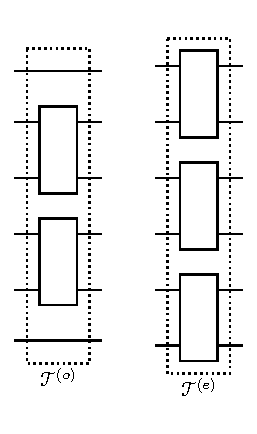
\includegraphics[width=0.22\linewidth]{figures/appendix/Todd_Teven.pdf}
    % \caption{Caption}
    % \label{fig:enter-label}
\end{figure}
The whole tensor network $\Twhole$ could be expressed by alternately apply $T^{(o)}$ and $T^{(e)}$ gates, 
\begin{equation}
\Twhole \left(t, b_1, b_2\right)=T^{(o)^{b_2}}\left(\prod_{i=0}^{t} T^{(e)} T^{(o)}\right) T^{(e)^{b_1}}, 
\end{equation}
where $b_1, b_2 \in\{0,1\}$, $t+b_1+b_2$ stands for the number of layers.


The calculation of $\alpha_{S,d}$ could be represented by the tensor network contraction.
Notice the matrix identity 
\begin{equation}
    \ketbra{0} = \frac{1}{2^n} \sum_{\Lambda\subset [2n]} \prod_{i \in \Lambda} Z_i,
\end{equation}
where $Z_i$ denotes the application of the Pauli Z operator to the $i$-th qubit.
Specially, let $\prod_{i \in \emptyset} Z_i = \mathbb{I}_n$. Then, the super vector of $\supket{0,0}$ could be expressed as
\begin{equation}
\label{eq: zz anonymous 6}
    \supket{0,0} = \frac{1}{2^{2n}} \sum_{\Lambda, \Lambda' \subset [2n]}  \supket{\prod_{i \in \Lambda }  Z_i, \prod_{j \in \Lambda'} Z_j}.
\end{equation}
By transforming all the super vectors and the super operators in the Pauli basis, 
the evolution of $\mathcal{U}_Q \supket{\gamma_S}$ could be equivalently expressed by 
\begin{equation}
\label{eq: transfer evolution of U to tensor}
    \int \dd\mu(Q) \mathcal{U}_Q^{\otimes 2} \supket{\gamma_S,\gamma_S} = \Twhole \supket{P^S}.
\end{equation}
In the equation, for simplicity, we slightly abuse the notation $\supket{P^S}$ to represent the tensor of Pauli basis $\supket{P^S, P^S}$. Formally, $\supket{P^S}$ is the tensor $\delta_{S}^{R}$, where $\delta_{S}^{R}=1$ if and only if $R=S$, otherwise, $\delta_{S}^{R}=0$. In this representation, The tensor contraction $\Twhole(t, b_1, b_2) P^S$ is equivalent to the evolution $\int \dd\mu(Q) \mathcal{U}_Q^{\otimes 2} \supket{\gamma_S,\gamma_S}$. Thus, the calculation of $\alpha_{S,d}$ could be expressed as the tensor network contraction, as illustrated in Fig.~\ref{fig:TNcoefRep}. \textcolor{cyan}{polish the figure}
\begin{figure}
    \centering
    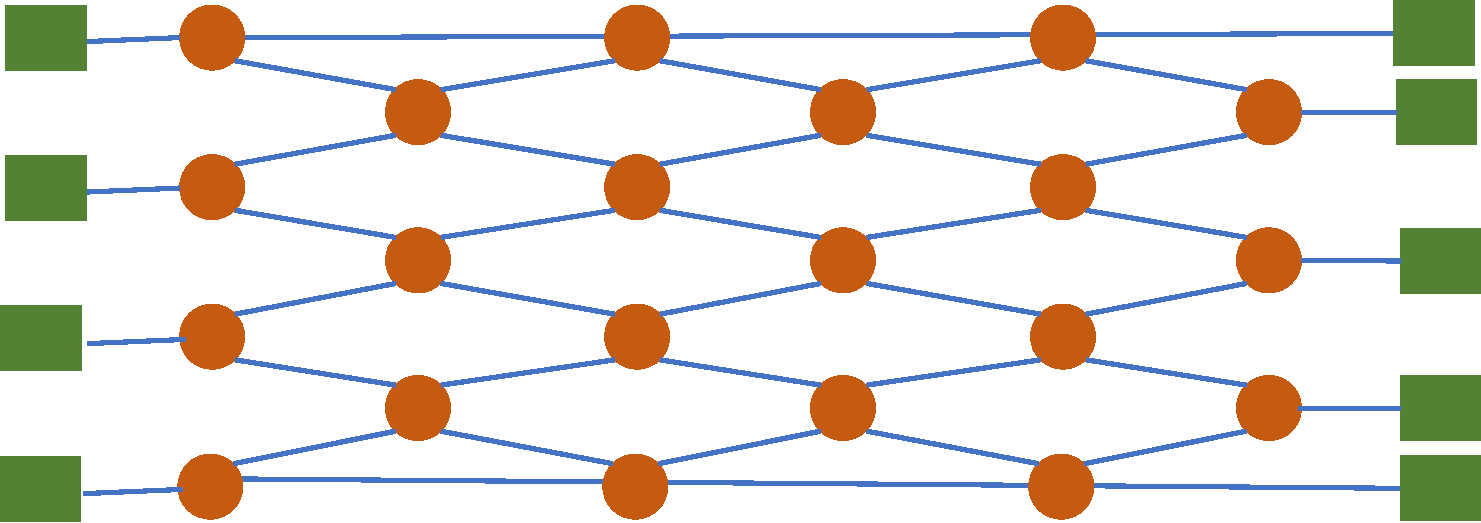
\includegraphics[width = 0.8\textwidth]{shallowCStensor_rep.pdf}
    \caption{Tensor network representation of the twirled $d$-layers matchgate circuit.}
    \label{fig:TNcoefRep}
\end{figure}






\begin{lemma}[Theorem 1 in \cite{wan2022matchgate}]
    Let $Q$ be a matrix uniformly randomly sampled from orthogonal group $\mathcal{O}(n)$, then
\begin{align}
& \int_{Q\sim M_n} \dd\mu(Q) \mathcal{U}_Q = \supket{\mathbb{I}}\supbra{\mathbb{I}}\\
& \int_{Q\sim M_n} \dd\mu(Q)\mathcal{U}_Q^{\otimes 2} = \sum_{k=0}^{2n}\supket{\mathcal{R}_k^{(2)}}\supbra{\mathcal{R}_k^{(2)}}\\
& \int_{Q\sim M_n} \dd\mu(Q)\mathcal{U}_Q^{\otimes 3} = \sum_{
\substack{
k_1,k_2,k_3\geq 0\\
k_1 + k_2 + k_3\leq 2n
}
}\supket{\mathcal{R}_{k_1,k_2,k_3}^{(3)}}\supbra{\mathcal{R}_{k_1,k_2,k_3}^{(3)}}.
\end{align}
where
\begin{align}
    &\supket{\mathcal{R}_k^{(2)}} = { 2n\choose k}^{-1/2} \sum_{S\subseteq [2n],|S|=k}\supket{\gamma_S}\supket{\gamma_S}\\
    &\supket{\mathcal{R}_k^{(3)}} = {2n \choose k_1,k_2,k_3,2n-k_1-k_2-k_3}^{-1/2} \sum_{
    \substack{
 S_1, S_2, S_3\subseteq [2n] disjoint\\
 \abs{S_j}=k_j,1\leq j\leq 3
    }
    } \supket{\gamma_{S_1}\gamma_{S_2}}
    \supket{\gamma_{S_2}\gamma_{S_3}}
    \supket{\gamma_{S_3}\gamma_{S_1}}
\label{eq:third_moment}
\end{align}
\label{lem:threemomentsMatchgate}
\end{lemma}

\begin{lemma}
\label{lemma: The net phase of alpha is 1}
    The net phase of $\alpha_{S,d}$ is $1$.
\end{lemma}
\begin{proof}
    The net phase of $\alpha_{S,d}$ is $1$ is $(-1)^{\frac{|S|(|S|-1)}{2}} (-1)^{\floor{|S|/2}}$. We categorize the discussion of the parity of $|S|$.
    \begin{enumerate}
        \item \textbf{$|S|$ is an odd number.} Let $|S| = 2q+1$, $ q\in \mathbb{N}$, $q\geq 0$. And then
        \begin{equation}
            (-1)^{\frac{|S|(|S|-1)}{2}} (-1)^{\floor{|S|/2}} = (-1)^{q(2q+1)+q} = 1.
        \end{equation}
        \item \textbf{$|S|$ is an even number.} Let $|S| = 2q$, $ q\in \mathbb{N}$, $q\geq 0$. And then
        \begin{equation}
            (-1)^{\frac{|S|(|S|-1)}{2}} (-1)^{\floor{|S|/2}} = (-1)^{(2q-1)q+q} = 1.
        \end{equation}
    \end{enumerate}
\end{proof}

\begin{table}
\centering
\begin{tabular}{|c|c|c|c|c|c|c|c|c|c|c|c|c|c|c|c|c|}
	\hline
	T  &II &IX &IY &IZ &XI &XX &XY &XZ &YI &YX &YY &YZ &ZI &ZX &ZY &ZZ \\ \hline
    II & 1 &   &   &   &   &   &   &   &   &   &   &   &   &   &   &   \\ \hline
    IX &   &1/4&1/4&   &   &   &   &1/4&   &   &   &1/4&   &   &   &   \\ \hline
    IY &   &1/4&1/4&   &   &   &   &1/4&   &   &   &1/4&   &   &   &   \\ \hline
    IZ &   &   &   &1/6&   &1/6&1/6&   &   &1/6&1/6&   &1/6&   &   &   \\ \hline
    XI &   &   &   &   &1/4&   &   &   &1/4&   &   &   &   &1/4&1/4&   \\ \hline
    XX &   &   &   &1/6&   &1/6&1/6&   &   &1/6&1/6&   &1/6&   &   &   \\ \hline
    XY &   &   &   &1/6&   &1/6&1/6&   &   &1/6&1/6&   &1/6&   &   &   \\ \hline
    XZ &   &1/4&1/4&   &   &   &   &1/4&   &   &   &1/4&   &   &   &   \\ \hline
    YI &   &   &   &   &1/4&   &   &   &1/4&   &   &   &   &1/4&1/4&   \\ \hline
    YX &   &   &   &1/6&   &1/6&1/6&   &   &1/6&1/6&   &1/6&   &   &   \\ \hline
    YY &   &   &   &1/6&   &1/6&1/6&   &   &1/6&1/6&   &1/6&   &   &   \\ \hline
    YZ &   &1/4&1/4&   &   &   &   &1/4&   &   &   &1/4&   &   &   &   \\ \hline
    ZI &   &   &   &1/6&   &1/6&1/6&   &   &1/6&1/6&   &1/6&   &   &   \\ \hline
    ZX &   &   &   &   &1/4&   &   &   &1/4&   &   &   &   &1/4&1/4&   \\ \hline
    ZY &   &   &   &   &1/4&   &   &   &1/4&   &   &   &   &1/4&1/4&   \\ \hline
    ZZ &   &   &   &   &   &   &   &   &   &   &   &   &   &   &   & 1 \\ \hline
\end{tabular}
\caption{Values of tensor $T$. The head of columns represents the input of $T$ while the head of rows represents the output of $T$. For example, the value in row `XY' and column `YZ' represent the value $T^{XY}_{~~YZ}$.  The blank space of the table stands for $0$.    }
\label{table: the 16x16 matrix of T}
\end{table}



\section{Simplify the tensor contraction for the case $|S|=2$}
We have changed the evaluation of the variance to focus on the tensor contraction of $\alpha_{S,d}$. Our main goal is to analyze how the order of $\alpha_{S,d}$ varies with the number of layers. However, estimating this order using tensor network contraction is challenging. Therefore, we will examine a specific case where $|S|=2$, which is the smallest non-trivial scenario. This simplification allows us to streamline the calculation of contraction and map the calculation to a different model.

%  Let $T^{(o)}$ be the odd layer of T gates, and $T^{(e)}$ be the even layer of T gates. Then we have the following circuits:


The evolution of $\mathcal{U}_Q \supket{\gamma_S}$ is limited to a subspace of the whole Hilbert space because the matchgate circuit conserves the cardinal number $|S|$. Thus, due to Eq.~\eqref{eq: transfer evolution of U to tensor}, the results of tensor contraction should obey the cardinal conservation as well
\begin{equation}
    \label{eq: zz anonymous 1}
    \Twhole (t, b_1,b_2)\supket{P^S}  = \sum_{|S'| = |S|} \xi_{S'} \supket{P^{S'}},
\end{equation}
where $S, S' \subset [2n]$, and $\xi_{S'}$ are real coefficient. 
Thus, its equivalent to study the tensor in the sub-representation of the space $\mathrm{span}\{\gamma_{S'} \mid |S'| = |S| \}$. This simplification can significantly reduce the complexity of the calculations.

% \begin{equation}
%     \label{eq: _anonymous 1}
%     \mathcal{U}_Q \supket{\gamma_S} = \sum_{|S'| = |S|} \xi_{S'} \supket{\gamma_{S'}}, 
% \end{equation}

% The evolution of $\mathcal{U}_Q \supket{\gamma_S}$ is limited to a subspace of the whole Hilbert space because the matchgate circuit conserves the cardinal number $|S|$, 
% \begin{equation}
%     \label{eq: _anonymous 1}
%     \mathcal{U}_Q \supket{\gamma_S} = \sum_{|S'| = |S|} \xi_{S'} \supket{\gamma_{S'}}, 
% \end{equation}
% where $S, S' \subset [2n]$, and $\xi_{S'}$ are real coefficient. The property will be held when we represent it with tensor network
% \begin{equation}
% \label{eq: _anonymous 2}
%     \Twhole \supket{P^S} = \sum_{|S'| = |S|} \xi'_{S'} \supket{P^{S'}}.
% \end{equation}
% In the equation, for simplicity, we slightly abuse the notation $\supket{P^S}$ to represent the tensor of Pauli basis $\supket{P^S, P^S}$. Formally, $\supket{P^S}$ is the tensor $\delta_{S}^{R}$, where $\delta_{S}^{R}=1$ if and only if $R=S$, otherwise, $\delta_{S}^{R}=0$. In this representation, The tensor contraction $\Twhole P^S$ is equivalent to the evolution $\int \dd\mu(Q) \mathcal{U}_Q^{\otimes 2} \supket{\gamma_S,\gamma_S}$.
% Thus, the 



% 引入|S|=2
Here, we focus on a specific circuit configuration that starts with an even-layer $T^{(e)}$ and ends with an odd-layer $T^{(o)}$, which means $b_1 = 1$ and $b_2 = 0$. The number of qubits in the circuit is set to be an even number. Additionally, the observable $\gamma_S$ is restricted to $|S|=2$. From the discussion about Eq.~\eqref{eq: zz anonymous 1}, the evolution could be restricted to the subspace $\mathrm{span}\{\gamma_i\gamma_j \mid i\neq j, 1\leq i,j \leq 2n \}$. By Jordan-Wigner transformation, the basis $\gamma_i\gamma_j$ obtains the form
% \begin{equation}
%     \begin{aligned}
        
%     \end{aligned}
% \end{equation}
\begin{equation}
\begin{aligned}
Z_l, \quad & X_l\left(\prod_{k=l+1}^{m-1} Z_k\right) X_m, \quad &X_l\left(\prod_{k=l+1}^{m-1} Z_k\right) Y_m, \\
& Y_l\left(\prod_{k=l+1}^{m-1} Z_k\right) X_m, \quad &Y_l\left(\prod_{k=l+1}^{m-1} Z_k\right) Y_m,
\end{aligned}
\end{equation}
where $1\leq l,m\leq 2n$.

% 现在要干什么
The representation $\mathrm{span}\{\gamma_i\gamma_j \mid i\neq j, 1\leq i,j \leq 2n \}$ could be reduced to a smaller subspace. From Table \ref{table: the 16x16 matrix of T}, we found that the value of tensor $T^{X, \cdot}_{~~\cdot, \cdot}$ and $T^{Y, \cdot}_{~~\cdot, \cdot}$ are always be the same. In other words, in the output of $\Twhole (t, b_1,b_2)\supket{P^S}$, the basis $\supket{\cdot, X, \cdot}$ and $\supket{\cdot, Y, \cdot}$ always simultaneously appear and have the same coefficients. Let 
\begin{equation}
    M_i := \frac{1}{\sqrt{2}}(X_i + Y_i),
\end{equation}
then, the subspace 
\begin{equation}
    V_{P} := \mathrm{span}\{\supket{Z_i}, \supket{M_i(\prod Z_k)M_j}\}
\end{equation}
is a sub-representation of $\Twhole$. In more precise, group representation theory language, $T^{(e)}V_P$ is a representation of the free group with generator $T^{(e)}T^{(o)}$. We interpret $\Twhole_{V}(t)(v)$ as the group element $(T^{(e)}_{V}T^{(o)}_{V})^t$ acts on the vector space $T^{(e)}_{V} (V)$, and $T^{(e)}_{V} (V) = V$ in specific cases. For simplicity, we will use informal language when there is no ambiguity.
Finally, the estimation of $\alpha_{S,d}$ could be simplified to calculate the tensor contraction in the space $V_P$.


\section{Reduce the calculation to polynomial space}
\begin{figure}
    \centering
    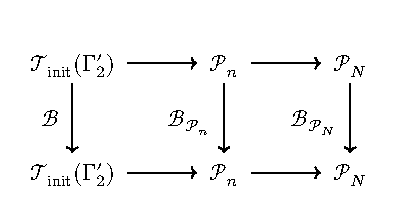
\includegraphics[width=0.8\linewidth]{figures/appendix/commute_diagram.pdf}
    \caption{The diagram shows how we simplify the calculation step by step. The horizontal arrows point from a high-dimensional space to a relatively low-dimensional space. The vertical arrows stand for the corresponding operators of $\Twhole(t,b_1, b_2)$ in different representations. Finally, we reduce it to the $N$-elementary polynomial of the $2$nd degree polynomial space.}
    \label{diagram: commute diagram}
\end{figure}

% We use polynomial space to represent $\Twhole$ because polynomial space obtains the properties we need, like multiplication and addition that we will use later.
We represent $\Twhole$ using polynomial space because it provides the essential properties we require, such as multiplication and addition, which will be important for our later work. 

Notice that the space $V_P$ is isometric to the $n$-elementary polynomial of the $2$nd degree polynomial space $\mathcal{P}_n$. The isometric could be constructed by the following
\begin{equation}
    \begin{aligned}
        \phi : V_P &\to \mathcal{P}_n \\
        \supket{M_i(\prod Z_k)M_j} &\mapsto x_i x_j \\
        \supket{Z_i} &\mapsto x_i^2.
    \end{aligned}
\end{equation}
The linear map $\phi$ is a homomorphism with inverse, which means it is an isometric between $V_P$ and $\mathcal{P}_n$. The equivalent representation of $\Twhole$ could be constructed by
\begin{equation}
    \Twhole_{\mathcal{P}_n}(t) (\cdot) := \phi \circ \Twhole(t,1,0) \circ \phi^{-1} (\cdot).
\end{equation}
% Thus, we build the equivalent representation $\mathcal{P}_n$ with group action $\Twhole_{\mathcal{P}_n}(t)$.
% which is shown in the second loop in the Fig.~\ref{diagram: commute diagram}. 
We could also transfer the input of $\Twhole$ to space $\mathcal{P}_n$,
\begin{equation}
    \gamma_{ij} \longrightarrow \supket{M_i(\prod Z_k)M_j} \xrightarrow{~~\phi~~} x_i x_j.
\end{equation}
Thus, the action of $d$-layer matchgate circuit on the $\gamma_{ij}$ is equivalent to the action of $\Twhole_{\mathcal{P}_n}(t)$ on the term $x_i x_j$. 
Due to Lemma \ref{lemma: reduce Pn to PN}, the action could be further simplify by finding a sub-representation $\mathcal{P}_N$ of representation $\mathcal{P}_n$, where $N$ equals to $\frac{n}{2}$. Recall that $n$ is an even number so $N$ is an integer. 

% By reducing the representation to the polynomial space $\mathcal{P}_N$, some patterns are revealed so that we could analysis it. 
Certain hidden patterns are revealed by reducing the representation to the polynomial space $\mathcal{P}_N$. Most of the main results are been proved in the $\mathcal{P}_N$. 
% Most of the main results are proved on the 


\begin{lemma}
    \label{lemma: reduce Pn to PN}
    The space $\mathcal{P}_N$ isometric to a sub-representation of $\mathcal{P}_n$.
\end{lemma}
\begin{proof}
    Define the map $\phi$ as
    \begin{equation}
        \begin{aligned}
            \phi : \mathcal{P}_N &\to \mathcal{P}_n \\
              y_i^2 &\mapsto x_{2i-1}^2+4 x_{2i-1} x_{2i}+x_{2i}^2\\
           y_i y_j &\mapsto  \left(x_{2i-1}+x_{2i}\right)\left(x_{2j-1}+x_{2j}\right).
        \end{aligned}
    \end{equation}
    We define the  $\phi$ as a linear function so that the definition of mapping on a basis induces the mapping on any element of the space
    \begin{equation}
        \phi(\sum \xi_{ij}y_i y_j) = \sum \xi_{ij}\phi(y_i y_j).
    \end{equation}
    Thus, the space $\phi(\mathcal{P}_N)$ is a linear subspace of $\mathcal{P}_n$. Because $\phi$ is an injection, there is a map $\phi': \mathcal{P}_n \to \mathcal{P}_N$ such that $\phi' \circ\phi$ is identity. 
    Define the group action $\Twhole_{\mathcal{P}_N}$ as 
    \begin{equation}
        \Twhole_{\mathcal{P}_N}(y_i y_j) := \phi' \circ \Twhole_{\mathcal{P}_n}\circ \phi(y_i y_j).
    \end{equation}
    Based on the definition of representation, we know that the space $\mathcal{P}_N$ with the group action $\Twhole_{\mathcal{P}_N}$ is a representation. 
    
    The next step is to show that such a representation $\Twhole_{\mathcal{P}_N}$ does not lose information. Formally, we need to prove that the representation $\mathcal{P}_n$ could be reduced to a sub-representation isometrics to $\mathcal{P}_N$. Naturally, we will consider whether the subspace $\phi(\mathcal{P}_N) $ will constitute a sub-representation. If it is true, the proof is done because $\phi(\mathcal{P}_N) \simeq \mathcal{P}_N$.

    By the definition of sub-representation, we need to prove
    \begin{equation}
    \label{eq: PN is a sub representation}
        \Twhole_{\mathcal{P}_n}(t)(\phi(\mathcal{P}_N)) \subset \phi(\mathcal{P}_N), ~~\forall t .
    \end{equation}
    The readers may recall that the formal representation is $T^{(e)}_{\mathcal{P}_n} \phi(\mathcal{P}_N)$ rather than $\phi(\mathcal{P}_N)$. Here, we remove the ambiguity by proving $T^{(e)}_{\mathcal{P}_n} \phi(\mathcal{P}_N) = \phi(\mathcal{P}_N)$. 
    By expanding the definition of $T^{(e)}_{\mathcal{P}_n}$, we could get the calculation of $T^{(e)}_{\mathcal{P}_n} \phi(y_i y_j)$ backs to the space $V_P$. Then, we will find that $T^{(e)}_{\mathcal{P}_n} \phi(y_i y_j) = \phi(y_i y_j)$ from the Table~\ref{table: the 16x16 matrix of T}. Thus, we have $T^{(e)}_{\mathcal{P}_n} \phi(\mathcal{P}_N) = \phi(\mathcal{P}_N)$.
 
    The statement \eqref{eq: PN is a sub representation} will be proved by induction.
    
     When $t=0$, $T^{(e)}_{\mathcal{P}_n} \phi(\mathcal{P}_N)\subset \phi(\mathcal{P}_N)$ is true.
     Suppose the statement is true for $t^*$, then we have
    \begin{equation}
        \Twhole_{\mathcal{P}_n}(t^*)(\phi(y_iy_j)) = \sum \xi_{lm} \phi(y_ly_m).
    \end{equation}
    And then
    \begin{align}
        \Twhole_{\mathcal{P}_n}(t^*+1)(\phi(y_i y_j)) =& 
        T^{(e)}_{\mathcal{P}_n}T^{(o)}_{\mathcal{P}_n} (\sum \xi_{lm} \phi(y_ly_m)) \\
        \label{eq: zz anonymous 2}
        =& \sum \xi_{lm} \delta_{lm}T^{(e)}_{\mathcal{P}_n}T^{(o)}_{\mathcal{P}_n} ( x_{2i-1}^2+4 x_{2i-1} x_{2i}+x_{2i}^2) \\
        \label{eq: zz anonymous 3}
        & + \sum \xi_{lm} (1-\delta_{lm})T^{(e)}_{\mathcal{P}_n}T^{(o)}_{\mathcal{P}_n}\left(\left(x_{2 i-1}+x_{2 i}\right)\left(x_{2 j-1}+x_{2 j}\right)\right)
    \end{align}
    We will prove Eq.~\eqref{eq: zz anonymous 2} is in the space $\phi(\mathcal{P}_N)$, while the same result of Eq.~\eqref{eq: zz anonymous 3} can be proved by the same method. Now, we will directly calculate this expression
    \begin{equation}
    \begin{aligned}
        \label{eq: zz anonymous 4}
        &T^{(e)}_{\mathcal{P}_n}T^{(o)}_{\mathcal{P}_n} ( x_{2i-1}^2+4 x_{2i-1} x_{2i}+x_{2i}^2) \\
        =& T^{(e)}_{\mathcal{P}_n}(\frac{1}{6}x_{2i-2}^2 + \frac{2}{3} x_{2i-2}x_{2i-1} + x_{2i-2}x_{2i}+x_{2i-2}x_{2i+1} \\
        &+\frac{1}{6} x_{2i-1}^2 + x_{2i-1}x_{2i} + x_{2i-1}x_{2i+1}  \\
        &+\frac{1}{6} x_{2i}^2 + \frac{2}{3} x_{2i}x_{2i+1} + \frac{1}{6}x_{2i+1}^2  )\\
        =& \frac{1}{36}x_{2i-3}^2 + \frac{1}{9} x_{2i-3}x_{2i-2} +\frac{5}{12} x_{2i-3}x_{2i-1}+ \frac{5}{12} x_{2i-3}x_{2i}  + \frac{1}{4} x_{2i-3}x_{2i+1} + \frac{1}{4} x_{2i-3}x_{2i+2}  \\
        &+ \frac{1}{36}x_{2i-2}^2 + \frac{5}{12} x_{2i-2}x_{2i-1}+ \frac{5}{12} x_{2i-2}x_{2i}  + \frac{1}{4} x_{2i-2}x_{2i+1} + \frac{1}{4} x_{2i-2}x_{2i+2}  \\
        &+ \frac{2}{9}x_{2i-1}^2 + \frac{8}{9} x_{2i-1}x_{2i} + \frac{5}{12} x_{2i-1}x_{2i+1} + \frac{5}{12} x_{2i-1}x_{2i+2}\\
        & + \frac{2}{9}x_{2i}^2 + \frac{5}{12} x_{2i}x_{2i+1} + \frac{5}{12} x_{2i}x_{2i+2}\\
        & + \frac{1}{36}x_{2i+1}^2  + \frac{1}{9} x_{2i+1}x_{2i+2}\\
        & + \frac{1}{36}x_{2i+2}^2 \\
        % =& \frac{1}{6} y_{i-1}^2 + \frac{5}{3} y_{i-1}y_{i} + y_{i-1}y_{i+1} + \frac{4}{3} y_{i}^2 + \frac{5}{3} y_{i-1}y_{i+1}  + \frac{1}{6} y_{i+1}^2
    \end{aligned}
    \end{equation}
    The result expression is in $\phi(\mathcal{P}_N)$ because we could find a polynomial $y$ in $\mathcal{P}_N$ such that $\phi(y)$ equals the result expression,
    \begin{align}
        y =& \frac{1}{6} y_{i-1}^2 + \frac{5}{3} y_{i-1}y_{i} + y_{i-1}y_{i+1} + \frac{4}{3} y_{i}^2 + \frac{5}{3} y_{i-1}y_{i+1}  + \frac{1}{6} y_{i+1}^2 \\
        \phi(y) =& T^{(e)}_{\mathcal{P}_n}T^{(o)}_{\mathcal{P}_n} ( x_{2i-1}^2+4 x_{2i-1} x_{2i}+x_{2i}^2)
    \end{align}
    Thus, we get that 
    \begin{equation}
        T^{(e)}_{\mathcal{P}_n}T^{(o)}_{\mathcal{P}_n} ( x_{2i-1}^2+4 x_{2i-1} x_{2i}+x_{2i}^2) \subset \phi(\mathcal{P}_N).
    \end{equation}
    Thus, Eq.~\eqref{eq: zz anonymous 4} is contained in the space $\phi(\mathcal{P}_N)$, which completes the proof.
\end{proof}


% By studying the property of $\Twhole$, we could find a sub-representation of $\mathcal{P}_n$. Firstly, we transfer the input of $\Twhole$ to space $\mathcal{P}_n$,
% \begin{equation}
%     \gamma_{ij} \longrightarrow \supket{M_i(\prod Z_k)M_j} \xrightarrow{~~\phi~~} x_i x_j.
% \end{equation}
% With Lemma we prove that the output of $\Twhole_{\mathcal{P}_n}(t)$ obtains the 

\section{Mapping the action of tensors to random walk}
\label{sec: mapping the action of tensors to random walk}

\newcommand{\teto}{T^{(e)}_{\mathcal{P}_N}T^{(o)}_{\mathcal{P}_N}}
The action of layers is the lazy-symmetry random walk on a 2D square lattice in most sites. To illustrate this point, we will begin with a specific example. Considering $1<i<N-1$ and $i+1<j\leq N$, the action of $\teto$ is
\begin{equation}
    \label{eq: zz anonymous 5}
    \teto (y_iy_j) = \left(\frac{1}{4} y_{i-1} + \frac{1}{2}y_i + \frac{1}{4} y_{i-1}\right)\left( \frac{1}{4} y_{j-1} + \frac{1}{2}y_j + \frac{1}{4} y_{j-1} \right).
\end{equation}
In this case, the action of $\teto$ can be viewed as first independently evolving $y_i$ and $y_j$ in a one-dimensional lattice, and then combining them,
\begin{equation}
\label{eq: separate evolution}
    \begin{aligned}
        y_i &\to \frac{1}{4} y_{i-1} + \frac{1}{2}y_i + \frac{1}{4} y_{i-1}\\
    y_j &\to \frac{1}{4} y_{j-1} + \frac{1}{2}y_j + \frac{1}{4} y_{j-1}.
    \end{aligned}
\end{equation}
% We find that this pattern appears in most sites $y_iy_j$. Thus, we could separately analyze the evolving behavior in one-degree polynomial space (one-dimensional lattice), and then analyze the difference between the true evolved polynomial and the combined polynomial.
We observe that this pattern appears in most sites $y_iy_j$. Therefore, we can analyze the evolving behavior separately in one-dimensional polynomial space (one-dimensional lattice). Afterward, we can examine the differences between the true evolved polynomial and the combined polynomial. This approach is the skeleton of estimating the order of tensor contraction. Now, we will make the above concepts more specific and more concrete.

\begin{figure}
    \centering
    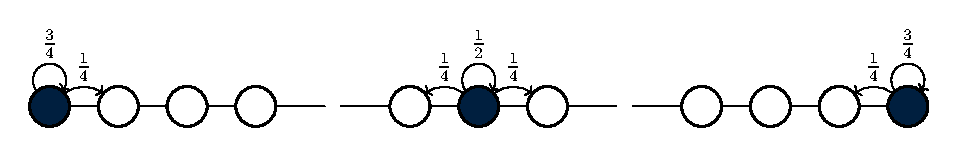
\includegraphics[width=0.95\linewidth]{figures/appendix/lazzy_symmetry_random_walk.pdf}
    \caption{Cases of lazy random walk. The circles represent the sites of the lattice $\{y_1, y_2, \cdots, y_n\}$, while the black circle stands for the starting site $y_i$, and the numbers over arrows are transition probability.}
    \label{fig: lazy random walk}
\end{figure}

We introduce the lazy-symmetry random walk in polynomial space, or the one-dimensional lattice, to describe the separate evolution behavior. A lazy-symmetry random walk is a type of Markov process, which is shown in Fig.~\ref{fig: lazy random walk}. In this process, consider a point located at a site $y_i$. In the next time interval, this point has a probability of $0.25$  moving to one of its neighboring sites $y_{i-1}$ or $y_{i+1}$, and it has a probability of $0.5$ staying in place. If the origin site is on the ends of the lattice, it has a probability of $0.75$ staying in place and has a probability of $0.25$ moving around. The probability transition relation could be expressed by 
\begin{equation}
\label{eq: lazy random walk L}
L\left(y_i\right)=
\begin{cases}
\frac{3}{4} y_1+\frac{1}{4} y_2, &i=1 \\
\frac{1}{4} y_{i-1}+\frac{1}{2} y_i+\frac{1}{4} y_{i+1}, &1<i<N \\
\frac{3}{4} y_N+\frac{1}{4} y_{N-1}, &i=N. 
\end{cases}
% \left\{\begin{array}{l}
% \end{array}\right.
\end{equation}
We could see that the separate evolution in Eq.~\eqref{eq: separate evolution} fits the form of lazy-symmetry random walk. 
% Thus, we could map the action of $\teto$ to a transition of random walk.


% In Eq.~\eqref{eq: zz anonymous 5}, we show the transition result of $\teto$ in a special case. Now, we show the transition results in any possible cases in Table.~\ref{table: transition table of teto}. The way how this table be generated is similar to Eq.~\eqref{eq: zz anonymous 4}. 

In Eq.~\eqref{eq: zz anonymous 5}, we showed the result of how $y_iy_j$ transfers in one specific situation. Now, we will show all possible results in any situation in Table \ref{table: transition table of teto}. The table lists all the possible transition results no matter what inputs it receives. 
It was created in a similar way to the previous example in Eq.~\eqref{eq: zz anonymous 4}. 
% This table provides a complete listing of all the potential changes to ηηο for all possible situations. This will help outline how the symbol may vary depending on whatever inputs it is given.




In Table \ref{table: transition table of teto}, we can see that in most cases 
\begin{equation}
    \teto(y_i y_j) = L(y_i) L(y_j)
\end{equation}
except for the cases when $|i-j|\leq 1$. 
Moreover, the coefficients of remainder terms $\teto(y_i y_j) - L(y_i)L(y_j)$ are small. Refs.~\cite{giuggioli2020exact} gives the analytical solution of lazy-symmetry random walk,
\begin{equation}
% \label{eq: propogator of lazy random walk}
     L^t(y_i) = \sum_\mu \mathcal{L}_{i}(\mu, t) y_\mu,
    % = \frac{1}{N} + \frac{2}{N} \sum_{k=1}^{N-1} \cos \left(\left(n-\frac{1}{2}\right) \frac{\pi k}{N}\right) \cos \left(\left(n_0-\frac{1}{2}\right) \frac{\pi k}{N}\right) \cos ^{2 t} \frac{\pi k}{2 N}.
\end{equation}
where $L^t(y_i)$ represents the outcome of random walking $t$ steps from $y_i$ according to the propagation rule $L$ in Eq.~\eqref{eq: lazy random walk L}, and the $\mathcal{L}_{i}(\mu, t)$ represents the probability of stopping at $y_\mu$ after $t$-steps random walking,
\begin{equation}
    \mathcal{L}_{i}(\mu, t) = \frac{1}{N} + \frac{2}{N} \sum_{k=1}^{N-1} \cos \left(\left(\mu-\frac{1}{2}\right) \frac{\pi k}{N}\right) \cos \left(\left(i-\frac{1}{2}\right) \frac{\pi k}{N}\right) \cos^{2 t} \left(\frac{\pi k}{2 N}\right).
\end{equation}
Thus, for the evolution that could be separated by $\teto(y_iy_j) = L(y_i) L(y_j)$, we could get the analytical solution results
\begin{align}
    \Twhole_{\mathcal{P}_N} (t) (y_i y_j) =& (\teto)^t (y_i y_j) \\
    =& L^t(y_i)L^t(y_j) + R(y_iy_j)\\
    \label{eq: zz anonymous 7}
    =&\sum_{\mu,\nu} \left(\mathscr{L}_{ij} (\mu, \nu, t) y_\mu y_\nu + \mathscr{R}_{ij} (\mu, \nu, t) y_\mu y_\nu\right),
    % \label{eq: zz anonymous 20}
\end{align}
where
\begin{equation}
    \mathscr{L}_{ij} (\mu, \nu, t) := \mathcal{L}_{i}(\mu, t)\mathcal{L}_{j}(\nu, t).
\end{equation}
The $R$ stands for the remind terms caused by the near-diagonal terms $y_i y_j$, $|i-j| \leq 1$ in Table \ref{table: transition table of teto}. 

\begin{table}
    \centering
    \renewcommand\arraystretch{2}
    \begin{tabular}{|c|l|}
        \hline$y_i y_j$ & $\teto (y_i y_j)$ \\
        \hline$i=j=1$ & $L(y_i)L(y_j) -\frac{5}{144} y_1 y_1-\frac{5}{144} y_2 y_2+\frac{5}{72} y_1 y_2$ \\
        \hline $1<i<N, j=i$ & $L(y_i)L(y_j)-\frac{5}{144} y_{i-1} y_{i-1}+\frac{1}{36} y_{i-1} y_i+\frac{1}                           {24} y_{i-1} y_{i+1}-\frac{1}{36} y_i y_i+\frac{1}{36} y_i y_{i+1}-\frac{5}{144} y_{i+1} y_{i+1}$ \\
        \hline $1 \leq i<N, j=i+1$ & $L(y_i)L(y_j)-\frac{1}{48} y_i y_i-\frac{1}{48} y_{i+1} y_{i+1}+\frac{1}{24} y_i y_{i+1}$ \\
        \hline$i=j=N$ & $L(y_i)L(y_j)-\frac{5}{144} y_N y_N-\frac{5}{144} y_{N-1} y_{N-1}+\frac{5}{72} y_{N-1} y_N$ \\
        \hline other case & $L(y_i)L(y_j)$ \\
        \hline
    \end{tabular}
    \caption{The transition result of $\teto$ with input $y_iy_j$ in different condition. Notice that $y_i y_j = y_j y_i$, the indices of the two factors $i$ and $j$ in term $y_iy_j$ can always be arranged in ascending order $i\leq j$.}
    \label{table: transition table of teto}
\end{table}


The calculation of $\alpha$ could be separated into two parts. The first part is contributed by the lazy-symmetry random walk, and the second part is contributed by the remind terms. Recall that the $\alpha_{S, d}$ can be calculated by the tensor contraction of $\Twhole$, $\supket{P^S}$ and $\supket{0,0}$. We have mapped the $\Twhole$ and $\supket{P^S}$ into polynomial space. And the $\supket{0,0}$ mapped into the polynomial space as well. Eq.~\eqref{eq: zz anonymous 6} has transformed $\supket{0,0}$ into Pauli basis. Notice that  $\supbra{Z_i}$ is a linear function which takes a super vector to a number. Especially, it takes $\supket{Z_i}$ to $1$ and takes the other Pauli basis to $0$. As we known, the $\supket{Z_i}$ is mapped to $x_i^2$ in $\mathcal{P}_n$. The derivative operators $\frac{\partial^2}{\partial x_i^2 }$ satisfy all these properties. 
In another word, The space of derivative operators is the dual space of polynomial space. 
Thus, we find the mapping from $\supket{Z_i}$ to $\mathcal{P}_n$
\begin{equation}
    \supket{Z_i} \to \frac{\partial^2}{\partial x_i^2 }.
\end{equation}
After some algebras, we map the $\supket{0,0}$ to $\mathcal{P}_N$ when $|S| = 2$
\begin{equation}
    \supket{0,0} \to \frac{1}{2^{2n}} \frac{1}{3} \sum_{i,j} \frac{\partial^2}{\partial y_i^2 }.
\end{equation}
Thus, the $\alpha_{S,2t+1}$ could be expressed as
\begin{equation}
    \alpha_{\{\gamma_i\gamma_j\},2t+1} = \frac{1}{3} \sum_{\mu} \frac{\partial^2}{\partial y_\mu^2 } \Twhole_{\mathcal{P}_N}(t) (y_i y_j).
\end{equation}
Then, we could calculate $\alpha_{S,d}$ in $\mathcal{P}_N$ via combining Eq.~\eqref{eq: zz anonymous 7}
\begin{align}
    \alpha_{\{\gamma_i\gamma_j\},2t+1} =& \frac{1}{3} \sum_\mu \mathscr{L}_{ij} (\mu, \mu, t) + \frac{1}{3} \sum_\mu \mathscr{R}_{ij} (\mu, \mu, t) \\
    =:& ~\alpl + \alpha_{\{\gamma_i\gamma_j\}, 2t+1}^{\mathscr{R}}.
    \label{eq: zz anonymous 24}
\end{align}

% Moreover ADD SOMETHING HERE

\section{Estimate the order of $\alpl$}

We have separated the calculation of $\alpha_{\{\gamma_i\gamma_j\},2t+1}$ into two parts in Sec.~\ref{sec: mapping the action of tensors to random walk}. In this section, we aim to estimate the order of the first part, $\alpl$.
\begin{theorem}
\label{theorem: order of alpha l}
    The $\alpl$ could be estimated by the following formula
    \begin{equation}
        3\alpl = \frac{N}{\sqrt{2\pi t}} (e^{-\frac{a^2}{2t}}+ e^{-\frac{b^2}{2t}}) + \frac{2N}{\sqrt{2\pi t}}(e^{-\frac{a^2+2N(N-a)}{2t}}+ e^{-\frac{b^2+2N(N-b)}{2t}}) + \mathcal{O}\left(e^{-\frac{\pi^2}{2}t}\right),
    \end{equation}
    where $a$ is defined as $|i-j|$ and $b$ is defined as $i+j-1$.
\end{theorem}


\begin{proof}
By Lemma ~\ref{lemma: simplification of alpha L}, we could simplify the expression of $\alpl$ into Eq.~\eqref{eq: alpha L}. Then, we absorb the $k=0$ into the summation
\begin{equation}
\label{eq: zz anonymous 13}
\begin{aligned}
3\alpl & =\frac{1}{N}+\frac{1}{N} \sum_{k=1}^{N-1}\left[\cos \left((i-j) \frac{k \pi}{N}\right)+\cos \left((i+j-1) \frac{k \pi}{N}\right)\right] \cos ^{4 t}\left(\frac{\pi k}{2 N}\right) \\
& =-\frac{1}{N}+\frac{1}{N} \sum_{k=0}^{N-1}\left[\cos \left((i-j) \frac{k \pi}{N}\right)+\cos \left((i+j-1) \frac{k \pi}{N}\right)\right] \cos ^{4 t}\left(\frac{\pi k}{2 N}\right).
\end{aligned}
\end{equation}
In this way, the summation over k will go through a complete cycle/period. This will allow us to utilize some useful properties regarding trigonometric summations.

% Here, we want to 
We want to express this summation as a better-handled integral for computation and analysis purposes. To achieve this, we need to take the following two steps. First, we find that directly turning this into an integral is still not easy to calculate, so we need to replace the term $\cos ^{4 t}\left(\frac{\pi k}{2 N}\right)$ to make the integral of the whole expression easier to calculate. Secondly, we need to estimate the error of this integral approximation.

Notice that the $e^{-2tx^2}$ is a good estimation of $\cos ^{4 t}\left(x\right)$
\begin{equation}
\begin{aligned}
& e^{-2 t x^2}-\cos ^{4 t}(x) \\
= & e^{-2 t x^2}-e^{-2 t x^2+O\left(t x^4\right)} \\
= & e^{-2 t x^2}\left(1-e^{O\left(t x^4\right)}\right) \\
\sim & \mathcal{O}\left(t x^4 e^{-2 t x^2}\right).
\end{aligned}
\end{equation}

Substitute $\cos ^{4 t}\left(\frac{\pi k}{2 N}\right)$ with $e^{-\frac{k^2 \pi^2 t}{2N^2}}$ in Eq.~\eqref{eq: zz anonymous 13}, we have 
\begin{align}
3\alpl& =-\frac{1}{N}+\frac{1}{N} \sum_{k=0}^{N-1} e^{-\frac{k^2 \pi^2 t}{2 N^2}}\left[\cos \left((i-j) \frac{k \pi}{N}\right)+\cos \left((i+j-1) \frac{k \pi}{N}\right)\right]+\mathcal{O}\left(e^{-\frac{\pi^2}{2}t}\right)\\
& =-\frac{1}{N}+\frac{1}{N} \sum_{k=0}^{\infty}e^{-\frac{k^2 \pi^2 t}{2 N^2}}\left[\cos \left((i-j) \frac{k \pi}{N}\right)+\cos \left((i+j-1) \frac{k \pi}{N}\right)\right]+\mathcal{O}\left(e^{-\frac{\pi^2}{2}t}\right).
\label{eq: zz anonymous 19}
\end{align}
In the second line, we expand the summation to infinity, and it will not introduce much of errors because 
\begin{align*}
    \sum_{k=N}^{\infty} e^{-\frac{k^2 \pi^2 t}{2 N^2}} =& e^{-\frac{\pi^2}{2}t}\sum_{k=0}^{\infty} e^{-\frac{k^2 \pi^2 t}{2 N^2}} \\
    \leq& e^{-\frac{\pi^2}{2}t}\sum_{k=0}^{\infty} e^{-\frac{k \pi^2 t}{2 N^2}} \\
    =& e^{-\frac{\pi^2}{2}t} \frac{e^{\frac{\pi^2 t}{2 N^2}}}{e^{\frac{\pi^2 t}{2 N^2}} -1 } \\
    =& \mathcal{O}\left(e^{-\frac{\pi^2}{2}t}\right)
\end{align*}
Lemma ~\ref{lemma: integral reminder} did the second job, which turns the summation to the integral and evaluate the errors. Then, we could calculate the summation of series in Eq.~\eqref{eq: zz anonymous 19} via Lemma ~\ref{lemma: integral reminder}
\begin{equation}
    3\alpl = \frac{N}{\sqrt{2\pi t}} (e^{-\frac{a^2}{2t}}+ e^{-\frac{b^2}{2t}})
    + \frac{2N}{\sqrt{2\pi t}}(e^{-\frac{a^2+2N(N-a)}{2t}}+ e^{-\frac{b^2+2N(N-b)}{2t}}) + \mathcal{O}\left(e^{-\frac{\pi^2}{2}t}\right),
    % \left( 1+ 2e^{-\frac{2N(N-a)}{t}} + \mathcal{O}(e^{-\frac{6N^2}{t}})\right).
\end{equation}
where $a$ is defined as $|i-j|$ and $b$ is defined as $i+j-1$. Here we absorb the error term given by Lemma ~\ref{lemma: integral reminder} into the $\mathcal{O}\left(e^{-\frac{\pi^2}{2}t}\right)$ in Eq.~\eqref{eq: zz anonymous 19}.

% Thus, $\alpl$ will be in order $\frac{1}{\mathrm{poly}(n)}$ if $t = \Theta(a^2)$. Otherwise, if $t = o(a^2)$, there is a exponential small factor $ e^{-\frac{a^2}{2t}}$ which makes $\alpl$ a smaller term in terms of order.

\end{proof}
We can therefore conclude that the value of $\alpl$ will be on the order of $\frac{1}{\mathrm{poly}(n)}$ if $t$ is of the same order magnitude as $a^2$, $t = \Theta(a^2)$. Alternatively, if $t$ is considered to be of lower order than $a^2$, as denoted by the little-o notation $t = o(a^2)$, then there exists an additional exponentially small term $ e^{-\frac{a^2}{2t}}$ present in the expression for $\alpl$.
\begin{lemma}
\label{lemma: simplification of alpha L}
The expression of $\alpl$ could be simplified to the following form
    \begin{equation}
    \label{eq: alpha L}
        3\alpl=\frac{1}{N}+\frac{1}{N} \sum_k\left[\cos \left((i-j) \frac{k \pi}{N}\right)+\cos \left((i+j-1) \frac{k \pi}{N}\right)\right] \cos ^{4 t}\left(\frac{\pi k}{2 N}\right).
    \end{equation}
\end{lemma}
\begin{proof}
    The lemma will be proved by directly calculation.

\begin{align}
    3\alpl =& \sum_\mu \left[ \frac{1}{N} + \frac{2}{N} \sum_{k=1}^{N-1} \cos \left(\left(i-\frac{1}{2}\right) \frac{\pi k}{N}\right) \cos \left(\left(\mu-\frac{1}{2}\right) \frac{\pi k}{N}\right) \cos ^{2 t} \left( \frac{\pi k}{2 N} \right)\right] \nonumber\\
     &\times\left[ \frac{1}{N} + \frac{2}{N} \sum_{l=1}^{N-1} \cos \left(\left(j-\frac{1}{2}\right) \frac{\pi l}{N}\right) \cos \left(\left(\mu-\frac{1}{2}\right) \frac{\pi l}{N}\right) \cos ^{2 t}\left( \frac{\pi l}{2 N} \right)  \right] \nonumber\\
     =& 1/N + \frac{2}{N^2} \sum_k \left[\sum_\mu \cos\left(\left(\mu-\frac{1}{2}\right) \frac{\pi k}{N}\right)  \right] 
     \cos \left(\left(i-\frac{1}{2}\right) \frac{\pi k}{N}\right) \cos ^{2 t} \left( \frac{\pi k}{2 N} \right) 
     \label{eq: zz anonymous 9}
     \\
     &+ \frac{2}{N^2} \sum_l \left[\sum_\mu \cos\left(\left(\mu-\frac{1}{2}\right) \frac{\pi l}{N}\right)  \right] 
     \cos \left(\left(i-\frac{1}{2}\right) \frac{\pi l}{N}\right) \cos ^{2 t} \left( \frac{\pi l}{2 N} \right) 
     \label{eq: zz anonymous 10}
     \\
     &+ \frac{4}{N^2} \sum_{k,l =1}^{N-1} \sum_{\mu = 1}^{N} \cos \left(\left(i-\frac{1}{2}\right) \frac{\pi k}{N}\right) \cos \left(\left(\mu-\frac{1}{2}\right) \frac{\pi k}{N}\right) \cos ^{2 t} \left( \frac{\pi k}{2 N} \right)  \nonumber\\
     &\times \cos \left(\left(j-\frac{1}{2}\right) \frac{\pi l}{N}\right) \cos \left(\left(\mu-\frac{1}{2}\right) \frac{\pi l}{N}\right) \cos ^{2 t}\left( \frac{\pi l}{2 N} \right)  
     \label{eq: calculation of alpha L}
\end{align}
% \begin{longdiv}
%     123 &= \\
% \end{longdiv}

Notice that the summation of cosin function is zero 
\begin{equation}
\begin{aligned}
\sum_{\mu=1}^{N} \cos\left(\left(\mu-\frac{1}{2}\right) \frac{\pi k}{N}\right)& =-\frac{1}{2} \cos \left(\frac{1}{2} \pi(2 k+1)\right) \csc \left(\frac{\pi k}{2 N}\right) \\
& =\sin (k \pi) \csc \left(\frac{\pi k}{2 N}\right) \\
& =0.
\end{aligned}
\end{equation}
Substitute this identity into Eq.~\eqref{eq: calculation of alpha L}, we could eliminate the terms in line \eqref{eq: zz anonymous 9} and \eqref{eq: zz anonymous 10}. 

Also, notice that
\begin{equation}
\label{eq: zz anonymous 12}
\begin{aligned}
& \sum_{\mu=1}^{N} \cos \left(\frac{\pi\left(\mu-\frac{1}{2}\right) i}{N}\right) \cos \left(\frac{\pi\left(\mu-\frac{1}{2}\right) j}{N}\right) \\
= & \frac{1}{2} \sum_{\mu=1}^{N} \cos \left(\frac{\pi\left(\mu-\frac{1}{2}\right) i}{N}-\frac{\pi\left(\mu-\frac{1}{2}\right) j}{N}\right)+\cos \left(\frac{\pi\left(\mu-\frac{1}{2}\right) i}{N}+\frac{\pi\left(\mu-\frac{1}{2}\right) j}{N}\right) \\
= & \frac{1}{2} \sum_{\mu=1}^{N} \cos \left(\frac{\pi(2 \mu-1)(i-j)}{2 N}\right)+\cos \left(\frac{\pi(2 \mu-1)(i+j)}{2 N}\right) \\
= & \frac{1}{4}\left(\sin (\pi(i+j)) \csc \left(\frac{\pi(i+j)}{2 N}\right)-\sin (\pi(j-i)) \csc \left(\frac{\pi(i-j)}{2 N}\right)\right).
\end{aligned}
\end{equation}
This result gets value $0$ when $\frac{\pi(i+j)}{2 N}\neq a \pi$ or $\frac{\pi(i-j)}{2 N}\neq b \pi$ for some integer $a$ and $b$, because $\sin(\pi m) = 0$. The term $ \sin(\pi m) \csc(\frac{\pi m}{2N})$ gets non-zero only when $\csc(\frac{\pi m}{2N})$ gets infinity. Then, we could write down the conditions that $i$ and $j$ satisfy
\begin{equation}
\left\{\begin{array}{l}
i+j=2 a N \text { or } |i-j|=2 b N \\
a, b \in \mathbb{Z} \\
1<i,j<N-1.
\end{array} \right.
\end{equation}
The equation shows that the result is $j=k$. We can use  L'Hôpital's rule to calculate the term
% As we known that
\begin{equation}
    \label{eq: zz anonymous 11}
    \lim_{x\to 0} \sin(\pi x) \csc(\frac{\pi x}{2N}) = 2N
\end{equation}
when $i$ and $j$ satisfy the condition $i=j$. Plugin Eq.~\eqref{eq: zz anonymous 11} and Eq.~\eqref{eq: zz anonymous 12} into Eq.~\eqref{eq: calculation of alpha L}, we have
\begin{equation}
    \label{eq: zz anonymous 13}
    \alpl = \frac{1}{N} + \frac{2}{N} \sum_k \cos \left(\left(i-\frac{1}{2}\right) \frac{\pi k}{N}\right)\cos \left(\left(j-\frac{1}{2}\right) \frac{\pi k}{N}\right)\cos ^{4 t}\left( \frac{\pi k}{2 N} \right).
\end{equation}
Finally, we use trigonometric identities to expand this equation, thereby completing this proof
\begin{equation}
    3\alpl=\frac{1}{N}+\frac{1}{N} \sum_k\left[\cos \left((i-j) \frac{k \pi}{N}\right)+\cos \left((i+j-1) \frac{k \pi}{N}\right)\right] \cos ^{4 t}\left(\frac{\pi k}{2 N}\right).
\end{equation}
\end{proof}

\begin{lemma}
\label{lemma: integral reminder}
The result of summing the infinite series is
    \begin{equation}
        \sum_0^\infty e^{-\frac{k^2\pi^2 t}{2N^2}} \cos(a\frac{\pi k}{N}) = \frac{N}{\sqrt{2\pi t}} e^{-\frac{a^2}{2t}}\left( 1+ 2e^{-\frac{2N(N-a)}{t}} + \mathcal{O}(e^{-\frac{6N^2}{t}})\right)+\frac{1}{2}
        % \sum_0^{\infty} f(n) = \frac{N}{\sqrt{2\pi t}} e^{-\frac{a^2}{2t}}\left( 1+ 2e^{-\frac{2N(N-a)}{t}} + \mathcal{O}(e^{-\frac{6N^2}{t}})\right)+\frac{1}{2}
    \end{equation}
    when $t<N^2$.
    % with remainder term $\Delta_a$ that satisfies 
    % \begin{equation}
    %     \Delta_a \leq e^{-\frac{a^2}{2t}}.
    % \end{equation}
\end{lemma}

\begin{proof}
To aid analysis, we define a new function $f(k)$ that captures the pattern of each term, where $f(k) = e^{-\frac{1}{2}\beta^2 k^2 t}\cos(a\beta k)$ and $\beta := \frac{\pi}{N}$. To determine the value of this infinite series, we invoke the Euler-Maclaurin formula. This formula relates the summation of a function to its integral representation, along with correction terms.

Specifically, the Euler-Maclaurin formula gives 
\begin{equation}
\label{eq: euler maclaurin expansion}
    \sum_{k=0}^{\infty} f(k)=\int_0^{\infty} f(x) d x+\frac{1}{2}+\int_0^{\infty} P_1(x) f^{\prime}(x) \dd x,
\end{equation}
where $P_1(x)=B_1(x-\lfloor x \rfloor)$, and $B_1$ is the first order Bernoulli polynomial
\begin{equation}
    B_1 = x-\frac{1}{2}.
\end{equation}
By applying this formula, we can express the infinite series summation in terms of integrals, facilitating further analysis and solution of the problem. 


Substitute the definition of $B_1$ into the Euler-Maclaurin expansion \eqref{eq: euler maclaurin expansion}, we have
\begin{align}
\sum_{k=0}^{\infty} f(k)=&\int_0^{\infty} f(x) \dd x+\frac{1}{2}-\frac{1}{2} \int_0^{\infty} f^{\prime}(x) \dd x+\int_0^{\infty}(x-\lfloor x\rfloor) f^{\prime}(x) \dd x
% =&\int_0^{\infty} f(x) \dd x+\frac{1}{2}-\frac{1}{2} (f(\infty) - f(0))+
% \sum_{k=0}^{\infty} \int_k^{k+1}(x-k) f^{\prime}(x) \dd x.
\label{eq: zz anonymous 15}
\end{align}
Integrating an serrate shape function can be relatively difficult. Therefore, we perform a Fourier transform on it, 
\begin{equation}
    x-\lfloor x\rfloor=\frac{1}{2}-\frac{1}{\pi} \sum_{k=1}^{\infty} \frac{1}{k} \sin (2 \pi k x).
\end{equation}
changing the integral of the serrate shape function into an integral of trigonometric functions. This makes the calculation simpler. 

By the definition of function $f$, the derivative of $f$ could be calculated
\begin{align}
f^{\prime}(x) & =-e^{-\frac{1}{2} t x^2 \beta^2} t x \beta^2 \cos [a x \beta]-a e^{-\frac{1}{2} t x^2 \beta^2} \beta \sin [a x \beta] \\
\label{eq: zz anonymous 14}
& =-t x \beta^2 f(x)-a \beta \tan (a x \beta) f(x). 
\end{align}
We utilize the symbolic computation platform Wolfram Mathematica to calculate the integral of $f(x)$
\begin{equation}
\label{eq: zz anonymous 17}
    \int_0^{\infty} f(x) \dd x = \frac{N}{\sqrt{2\pi t}} e^{-\frac{a^2}{2t}}
\end{equation}
and the integral of sin multiplied with $f'(x)$
\begin{equation}
    \int_0^{\infty} \sin (2 \pi k x) f^{\prime}(x) \dd x=-\frac{e^{-\frac{(2 k \pi+a \beta)^2}{2 t \beta^2}}\left(1+e^{\frac{4 a k \pi}{t^\beta}}\right) k \pi^{\frac{3}{2}}}{\sqrt{2 t \beta^2}}.
    \label{eq: zz anonymous 16}
\end{equation}
Plugin Eq.~\eqref{eq: zz anonymous 14}, Eq.~\eqref{eq: zz anonymous 16}, and Eq.~\eqref{eq: zz anonymous 17} to Eq.~\eqref{eq: zz anonymous 15}, we have 
\begin{align}
\sum_0^{\infty} f(n) & =\int_0^{\infty} f(x) \dd x+\frac{1}{2}+\sqrt{\frac{\pi}{2}} \sum_{k=1}^{\infty} \frac{e^{-\frac{(2 k \pi+a \beta)^2}{2 t \beta^2}}\left(1+e^{\frac{4 a k \pi}{t \beta}}\right)}{\sqrt{t \beta^2}} \\
& =\frac{N}{\sqrt{2\pi t}} e^{-\frac{a^2}{2t}}+\frac{1}{2}+N\sqrt{\frac{1}{2\pi t }}\left(\sum_{k=1}^{\infty} e^{-\frac{(2 k \pi+a \beta)^2}{2 t \beta^2}}+\sum_{k=1}^{\infty} e^{-\frac{(2 k \pi-a \beta)^2}{2 t \beta^2}}\right).
\label{eq: zz anonymous 18}
\end{align}

Now, we want to estimate the order of the third term in Eq.~\eqref{eq: zz anonymous 18}
\begin{align}
    \sum_{k=1}^{\infty} e^{-\frac{(2 k \pi+a \beta)^2}{2 t \beta^2}}+\sum_{k=1}^{\infty} e^{-\frac{(2 k \pi-a \beta)^2}{2 t \beta^2}} 
    \leq & 2\sum_{k=1}^{\infty} e^{-\frac{(2 k \pi-a \beta)^2}{2 t \beta^2}} \\
    =& 2 e^{-\frac{a^2}{2t}} \sum_{k=1}^{\infty} e^{-\frac{2 k^2 N^2-2kaN}{t}} \\
    \leq& 2 e^{-\frac{a^2}{2t} + \frac{2aN}{t}}\sum_{k=1}^{\infty} e^{-\frac{2 k^2 N^2}{t}} \\
    = &  2 e^{-\frac{a^2}{2t} + \frac{2aN}{t}} \left( e^{-\frac{2  N^2}{t}} + \mathcal{O}(e^{-\frac{6N^2}{t}}) \right).
\end{align}
If we consider $t$ to be smaller in order than $\mathcal{O}(N^2)$, then we can view $e^{-\frac{6N^2}{t}}$ as a small number.  Thus, the summation of $f(n)$ obtains the value
\begin{equation}
    \sum_0^{\infty} f(n) = \frac{N}{\sqrt{2\pi t}} e^{-\frac{a^2}{2t}}\left( 1+ 2e^{-\frac{2N(N-a)}{t}} + \mathcal{O}(e^{-\frac{6N^2}{t}})\right)+\frac{1}{2}.
\end{equation}

% We begin with 

% \begin{align}
% \label{eq: zz anonymous 16}
%     &\sum_{k=0}^{\infty} \int_k^{k+1}(x-k) f^{\prime}(x) \dd x \\
%     =&\frac{1}{4 \sqrt{t} \beta} e^{-\left(\frac{a^2}{2 t}\right)} \sum_{k=0}^{\infty}\left[2 e^{\frac{(a-\ii(1+k) t \beta)^2}{2 t}}\left(1+e^{2 \ii a(1+k) \beta}\right) \sqrt{t} \beta\right. \\
% & \left.+\sqrt{2 \pi}\left(\operatorname{erf}\left[\frac{\ii a+k t \beta}{\sqrt{2} \sqrt{t}}\right]-\operatorname{erf}\left[\frac{\ii a+(1+k) t \beta}{\sqrt{2} \sqrt{t}}\right] - \operatorname{erf}\left[\frac{\ii a- k t \beta}{\sqrt{2} \sqrt{t}}\right]+\operatorname{erf}\left[\frac{\ii a-(1+k) t \beta}{\sqrt{2} \sqrt{t}}\right]\right)\right].
% \end{align}
% In this derivation, we utilize the symbolic computation platform Wolfram Mathematica to simplify and transform the given expression. Mathematica allows us to systematically manipulate the terms in a rigorous, computational manner. 
% The $\operatorname{erf}$ stands for the integral of Gaussian integral
% \begin{equation}
%     \operatorname{erf}(z) := \frac{2}{\sqrt{\pi}}\int_0^z e^{-x^2} \dd x.
% \end{equation}
% Notice that the summation of $\operatorname{erf}\left[\frac{\ii a+k t \beta}{\sqrt{2} \sqrt{t}}\right]-\operatorname{erf}\left[\frac{\ii a+(1+k) t \beta}{\sqrt{2} \sqrt{t}}\right]$ obtains the pattern that the end of one term can be cancelled out by the beginning of the next term.
% \begin{equation}
%     \operatorname{erf}\left[\frac{\ii a}{\sqrt{2} \sqrt{t}}\right]-\operatorname{erf}\left[\frac{\ii a+ t \beta}{\sqrt{2} \sqrt{t}}\right] + \operatorname{erf}\left[\frac{\ii a+ t \beta}{\sqrt{2} \sqrt{t}}\right]-\operatorname{erf}\left[\frac{\ii a+2 t \beta}{\sqrt{2} \sqrt{t}}\right] + \operatorname{erf}\left[\frac{\ii a+2 t \beta}{\sqrt{2} \sqrt{t}}\right]-\operatorname{erf}\left[\frac{\ii a+3 t \beta}{\sqrt{2} \sqrt{t}}\right] + \cdots .
% \end{equation}

% Thus, the Eq.~\eqref{eq: zz anonymous 16} becomes 
% \begin{align}
%     &\sum_{k=0}^{\infty} \int_k^{k+1}(x-k) f^{\prime}(x) \dd x \nonumber \\
% = & \frac{1}{4} e^{-\left(\frac{a^2}{2 t}\right)} \sum_{k=0}^{\infty} 2 e^{\frac{(a-\ii(1+k) t \beta)^2}{2 t}}\left(1+e^{2 \ii a(1+k) \beta}\right) \\
% & +\frac{\sqrt{2 \pi}}{4 \sqrt{t} \beta} e^{-\left(\frac{a^2}{2 t}\right)}\left[\left(\operatorname{erf}\left[\frac{\ii a}{\sqrt{2} \sqrt{t}}\right]-\operatorname{erf}\left[\frac{\ii a+\infty}{\sqrt{2} \sqrt{t}}\right]\right)-\left(\operatorname{erf}\left[\frac{\ii a}{\sqrt{2} \sqrt{t}}\right] - \operatorname{erf}\left[\frac{\ii a-\infty }{\sqrt{2} \sqrt{t}}\right]\right)\right] \\
% = & \frac{1}{2} e^{-\left(\frac{a^2}{2 t}\right)} \sum_{k=0}^{\infty}\left(e^{\frac{(a-\ii(1+k) t \beta)^2}{2 t}}+e^{\frac{(a+\ii(1+k) t \beta)^2}{2 t}}\right)-\frac{\sqrt{2 \pi}}{2 \sqrt{t} \beta} e^{-\left(\frac{a^2}{2 t}\right)}.
% % = & \frac{1}{2} e^{-\left(\frac{a^2}{2 t}\right)} \frac{\sqrt{\frac{\pi}{2}}}{\sqrt{t} \beta}-\frac{\sqrt{2 \pi}}{2 \sqrt{t} \beta} e^{-\left(\frac{a^2}{2 t}\right)}+\Delta_a
% \end{align}
% Notice that
% \begin{align}
%     &\sum_{k=0}^{\infty} (e^{\frac{(a-\ii(1+k) t \beta)^2}{2 t}}+e^{\frac{(a+\ii(1+k) t \beta)^2}{2 t}}) \\
%     =& \sum_{k=0}^{\infty} (e^{\frac{(a-\ii k t \beta)^2}{2 t}}+e^{\frac{(a+\ii k t \beta)^2}{2 t}}) - 2e^{\frac{a^2}{2 t}} \\
%     =& e^{\frac{a^2}{2 t}}\sum_{k=0}^{\infty} e^{-\frac{k^2  \beta^2 t}{2 }}(e^{-\ii a k  \beta}+e^{\ii a k \beta}) - 2e^{\frac{a^2}{2 t}}\\
%     =& 2e^{\frac{a^2}{2 t}}\sum_{k=0}^{\infty} e^{-\frac{k^2  \beta^2 t}{2 }}\cos(a\beta k) - 2e^{\frac{a^2}{2 t}} \\
%     =& 2e^{\frac{a^2}{2 t}}\sum_{k=0}^{\infty} f(k) - 2e^{\frac{a^2}{2 t}}
% \end{align}


% Similarly, we 

\end{proof}


\section{The relation between $\alpl$ and $\alpr$}
Recall that we have divided the calculation of $\alpha_{\{\gamma_i\gamma_j\}, 2t+1}$ into two parts. One is the $\alpl$ and the other is $\alpr$. Theorem \ref{theorem: order of alpha l} gives the order of $\alpl$. In this section, we aim to bound the $\alpr$ by $\alpl$, so that the order of $\alpha_{\{\gamma_i\gamma_j\}, 2t+1}$ could be given by the $\alpl$.

We begin with the polynomial in Eq.~\eqref{eq: zz anonymous 7}
\begin{equation}
\label{eq: zz anonymous 21}
    \Twhole_{\mathcal{P}_N} (t) (y_i y_j) 
    =\sum_{\mu,\nu} \left(\mathscr{L}_{ij} (\mu, \nu, t) y_\mu y_\nu + \mathscr{R}_{ij} (\mu, \nu, t) y_\mu y_\nu\right).
\end{equation}
Then, we let the polynomial transform one time-interval step, and we get
\begin{align}
    &\Twhole_{\mathcal{P}_N} (t+1) (y_i y_j) \\
    =& \teto\left(\Twhole_{\mathcal{P}_N} (t) (y_i y_j)\right) \\
    =& \sum_{\mu,\nu} \left(\mathscr{L}_{ij} (\mu, \nu, t) (L(y_\mu) L(y_\nu) + R(y_\mu, y_\nu)) + \mathscr{R}_{ij} (\mu, \nu, t) (L(y_\mu) L(y_\nu) + R(y_\mu, y_\nu))\right)\\
    =& \sum_{\mu,\nu} \left(\mathscr{L}_{ij} (\mu, \nu, t) (L(y_\mu) L(y_\nu) + R(y_\mu, y_\nu)) + \mathscr{R}_{ij} (\mu, \nu, t) (L(y_\mu) L(y_\nu) + R(y_\mu, y_\nu))\right)\\
    =& \sum_{\mu,\nu} \mathscr{L}_{ij} (\mu, \nu, t+1) y_\mu y_\nu +  \sum_{\mu,\nu}\mathscr{L}_{ij} (\mu, \nu, t) R(y_\mu, y_\nu) \nonumber\\
    & + \sum_{\mu,\nu}\mathscr{R}_{ij} (\mu, \nu, t) (L(y_\mu) L(y_\nu) + R(y_\mu, y_\nu)).
    \label{eq: zz anonymous 22}
\end{align}
Deduce from Eq.~\eqref{eq: zz anonymous 21}, we have
\begin{equation}
    \label{eq: zz anonymous 23}
    \Twhole_{\mathcal{P}_N} (t+1) (y_i y_j) 
    =\sum_{\mu,\nu} \left(\mathscr{L}_{ij} (\mu, \nu, t+1) y_\mu y_\nu + \mathscr{R}_{ij} (\mu, \nu, t+1) y_\mu y_\nu\right). 
\end{equation}
Compare Eq.~\eqref{eq: zz anonymous 22} and Eq.~\eqref{eq: zz anonymous 23}, we have 
\begin{align}
    &\sum_{\mu,\nu} \mathscr{R}_{ij} (\mu, \nu, t+1) y_\mu y_\nu = \sum_{\mu,\nu}\mathscr{L}_{ij} (\mu, \nu, t) R(y_\mu, y_\nu) + \sum_{\mu,\nu}\mathscr{R}_{ij} (\mu, \nu, t) (L(y_\mu) L(y_\nu) + R(y_\mu, y_\nu)) \\
    &\mathscr{R}_{ij} (l, k, t+1) =  \sum_{\mu,\nu}\mathscr{R}_{ij} (\mu, \nu, t) \frac{\partial^2L(y_\mu) L(y_\nu)}{\partial y_l \partial y_k} + \sum_{\mu,\nu}\left( \mathscr{L}_{ij} (\mu, \nu, t) + \mathscr{R}_{ij} (\mu, \nu, t) \right)\frac{\partial^2 R(y_\mu, y_\nu)}{\partial y_l \partial y_k}.
    \label{eq: strict recursive relation}
\end{align}
Eq.~\eqref{eq: strict recursive relation} describes the strict relationship between $\mathscr{R}_{ij}$ and $\mathscr{L}_{ij}$ in a recursive form, thereby giving the relationship between $\alpl$ and $\alpr$. However, deriving the general term formula from this recursive formula is difficult. Therefore, we hope to use some inequalities to simplify this recursive relationship and thus bound $\alpr$ by $\alpl$.

We will first define some auxiliary variables, 
\begin{align*}
\alpha_k(t) & :=\frac{1}{2} \sum_{\mu=1}^{N-k}\left(\mathcal{L}_i(\mu, t) \mathcal{L}_j(\mu+k, t)+\mathcal{L}_i(\mu+k, t) \mathcal{L}_j(\mu, t)\right) \\
\beta_k(t) & :=\frac{1}{2} \sum_{\mu=1}^{N-k}\left(\mathscr{R}_{i, j}(\mu, \mu+k, t)+\mathscr{R}_{i, j}(\mu+k, \mu, t)\right) \\
a(t) & :=\binom{\alpha_0(t)}{\alpha_1(t)}, \quad b(t):=\binom{\beta_0(t)}{\beta_1(t)}.
\end{align*}
Notice that $3\alpl = \alpha_0(t)$, $3\alpr = \beta_0(t)$. Because $\mathscr{L}_{i, j}(\mu, \nu, t) + \mathscr{R}_{i, j}(\mu, \nu, t)$ represents the probability of being in site $y_iy_j$ during a random walk, it satisfies the property that the summation across all sites is $1$. Meanwhile, the summation of all $\mathscr{L}_{i, j}(\mu, \nu, t)$ is $1$. The two things deduce that
\begin{equation}
    \sum_{\mu, \nu} \mathscr{R}_{i, j}(\mu, \nu, t) =0.
\end{equation}
Especially, in numerical simulation, we observe that all $\mathscr{R}_{i, j}(\mu, \nu, t)$ are greater than $0$ except for $\mu=\nu$. Under this assumption, we have the following theory:
\begin{theorem}
\label{theorem: relation between alpha L and alpha R}
    Assume that $\mathscr{R}_{i, j}(\mu, \mu, t)<0$, and $\forall \mu \neq \nu$, $\mathscr{R}_{i, j}(\mu, \mu, t)>0$. $-\beta_0(t) \leq $.
\end{theorem}
% Theorem \ref{theorem: relation between alpha L and alpha R} gives the relationship  between $\alpl$ and $\alpr$. Combining with Eq.~\eqref{eq: zz anonymous 24}, we could get the order of $\alpha$.
Theorem \ref{theorem: relation between alpha L and alpha R} establishes the mathematical relationship between the two components $\alpl$ and $\alpr$. By combining this theoretical relationship with the equality described in Eq.~\eqref{eq: zz anonymous 24}, we are able to deduce the order of magnitude of the $\alpha_{\{\gamma_i\gamma_j\}, 2t+1}$. Bringing these pieces together allows us to systematically determine the scale or size of $\alpha_{\{\gamma_i\gamma_j\}, 2t+1}$ based on the other defined quantities. 



\begin{proof}[proof of theorem \ref{theorem: relation between alpha L and alpha R}]
   From the recursive relationship in Eq.~\eqref{eq: strict recursive relation} and Table \ref{table: transition table of teto}, we could write down the recursive relationship of $\beta_k$
   \begin{align}
    \beta_0(t+1) & \geq \frac{6}{16} \beta_0(t)+\frac{8}{16} \beta_1(t) + \frac{2}{16}\beta_2(t)-\frac{14}{144}\left(\beta_0(t)+\alpha_0(t)\right)-\frac{1}{24}\left(\beta_1(t)+\alpha_1(t)\right)\nonumber\\
    & + \frac{4}{16}(\mathscr{R}_{i j}(0,0, t-1) + \mathscr{R}_{i j}(N,N, t-1)) -  \frac{1}{16}(\mathscr{R}_{i j}(0,1, t-1) + \mathscr{R}_{i j}(1,0, t-1))\nonumber\\
    &- \frac{1}{16}(\mathscr{R}_{i j}(N-1,N, t-1) + \mathscr{R}_{i j}(N,N-1, t-1))\nonumber\\
    & \geq \frac{5}{18} \beta_0(t)+\frac{11}{24} \beta_1(t)-\frac{7}{72} \alpha_0(t)-\frac{1}{12} \alpha_1(t) \\
    & \geq \frac{5}{18} \beta_0(t)+\frac{5}{24} \beta_1(t)-\frac{7}{72} \alpha_0(t)-\frac{1}{12} \alpha_1(t) 
    % \beta_1(t+1) & \leq \frac{5}{9} \beta_0(t)+\frac{5}{12} \beta_1(t)-\frac{1}{18} \alpha_0(t)-\frac{1}{24} \alpha_1(t)
    \end{align}
    Here, we use the property that $\beta_0(t)+\alpha_0(t)$ is the summation of properties so that it is greater than $0$ to inequality deflate the terms at the edges, like $y_0y_0$ or $ y_0y_1$. Recall that we hold the assumption that $\mathscr{R}_{i, j}(\mu, \mu, t)<0$, and $\forall \mu \neq \nu$, $\mathscr{R}_{i, j}(\mu, \mu, t)>0$, so the edges terms of $\mathscr{R}_{i j}$ could be deflated out as well. Similarly, we have
    \begin{equation}
        \beta_1(t+1)  \geq \frac{5}{9} \beta_0(t)+\frac{5}{12} \beta_1(t)+\frac{1}{18} \alpha_0(t)+\frac{1}{24} \alpha_1(t).
    \end{equation}
    
    Let $\beta_0'$ and $\beta_1'$ obtains the above recursive relation
    \begin{equation}
        \begin{cases}
            \beta_0'(t+1) =& \frac{5}{18} \beta_0(t)+\frac{5}{24} \beta_1(t)-\frac{7}{72} \alpha_0(t)-\frac{1}{12} \alpha_1(t) \\
        \beta_1'(t+1)  =& \frac{5}{9} \beta_0(t)+\frac{5}{12} \beta_1(t)+\frac{1}{18} \alpha_0(t)+\frac{1}{24} \alpha_1(t)
        \end{cases}
        \label{eq: zz anonymous 25}
    \end{equation}
    with the same first term $\beta_0'(0) = \beta_0(0)$ and $\beta_1'(0) = \beta_1(0)$. The $\beta$ and $\beta'$ satisfy the relationship
    \begin{equation}
        \beta_0'(t) \geq \beta_0(t),\quad  \beta_1'(t) \geq \beta_1(t).
    \end{equation}
    Similarly, we denote $b'$ as $b'(t):=\binom{\beta_0'(t)}{\beta_1'(t)}$,
    % \begin{equation}
    % a'(t):=\binom{\alpha_0'(t)}{\alpha_1'(t)}, \quad b'(t):=\binom{\beta_0'(t)}{\beta_1'(t)}.
    % \end{equation}
    
    We rewrite the inequality groups \eqref{eq: zz anonymous 25} to the matrix form
    \begin{align}
        b^{\prime}(t+1)=C_b b^{\prime}(t)+C_a a(t), \quad \text{where}\\
        C_b=\left(\begin{array}[15pt]{c c}
        \frac{5}{18} & \frac{5}{24} \\ 
        \frac{5}{9} & \frac{5}{12}
        \end{array}\right), \quad C_a=\left(\begin{array}{cc}
        -\frac{7}{72} & -\frac{1}{12} \\
        \frac{1}{18} & \frac{1}{24}
        \end{array}\right),
    \end{align}
    and the matrices $C_b$ and $C_a$ govern these recursive dynamics. To solve this recursion explicitly, we diagonalize the $C_b$ matrix. This allows us to express the recursion in closed form,
    \begin{align}
    b'(t)=C_b^t b'(0)+\sum_{k=0}^{t-1}C_b^kC_aa(t-k-1).
    \end{align}
The term $C_b^t$ could be calculated by eigenvalue decomposition $C_b=Q \Lambda Q^{-1}$, where $\Lambda=\text{diag}(\frac{25}{36},0)$. The eigenvector corresponding to $\frac{25}{36}$ is $(2, \frac{3}{2})^T$. This allows us to express $C_b^k$ and $C_b^kC_a$ in terms of eigenvalues and eigenvectors
\begin{align}
    C_b^k=&\left(\frac{5}{6}\right)^{2k}\begin{pmatrix}
2 & \frac{3}{2} \\
0 & 0
\end{pmatrix}\\
C_b^kC_a =& \frac{1}{5}\left(\frac{5}{6}\right)^{2k}\begin{pmatrix}
-\frac{1}{9} & -\frac{5}{48} \\
% \frac{2}{9} & \frac{5}{24}
0 & 0
\end{pmatrix}
\end{align}
for any $k>0$. 

The variables we care about are $\alpha_0$ and $\beta_0$ because they are directly related to the $\alpl$ and $\alpr$. Thus, we mainly consider the first item of $C_b^t b'(0)$ and $C_b^kC_aa(t-k-1)$, which could be expressed in the following form
\begin{equation}
    C_b^kC_aa(t-k-1) = \lambda_k \alpha_0(t-k-1)+\eta_k \alpha_1(t-k-1).
\end{equation}
The $\lambda_k$ and the $\eta_k$ are coefficients 
\begin{equation}
    \begin{array}{ll}
\lambda_k=-\frac{1}{45}\left(\frac{5}{6}\right)^{2 k}, & \eta_k=-\frac{1}{48}\left(\frac{5}{6}\right)^{2 k}, \quad \forall k>0,  \\
\lambda_0=-\frac{7}{72}, & \eta_0=-\frac{1}{12}.
\end{array}
\end{equation}

Building on the previous relationships, we can now derive an explicit formula for $\beta'_0(t)$. From the expression for the first element of $C_b^kC_aa(t-k-1)$, we obtain
\begin{equation}
    \beta_0^{\prime}(t)=\sum_{k=0}^t\left(\lambda_k \alpha_0(t-k-1)+\eta_k \alpha_1(t-k-1)\right)
    \label{eq: zz anonymous 26}
\end{equation}
We also know from the recursive relation of $\mathcal{L}_i$ that the state variables satisfy
\begin{equation}
\alpha_0(t+1) \geq \frac{3}{8} \alpha_0(t)+\frac{1}{2} \alpha_1(t).
\end{equation}
Leveraging this inequality into Eq.~\ref{eq: zz anonymous 26} allows us to place an upper bound on $\beta'_0(t)$
\begin{align}
-\beta_0^{\prime}(t) \leq & -\sum_{k=1}^t\left(\lambda_k-\frac{3}{4} \eta_k+2 \eta_{k+1}\right) \alpha_0(t-k-1)+ \frac{19}{72} \alpha_0(t) - \frac{1}{16}\alpha_0(t-1) \\
\leq & \sum_{k=1}^t\left(\frac{5}{6}\right)^{2 k} \frac{307}{8640} \alpha_0(t-k-1)+ \frac{19}{72} \alpha_0(t) - \frac{1}{16}\alpha_0(t-1) \\
\leq & \frac{25}{72} \max _{k \geq 0}\left\{\alpha_0(t-k)\right\}
\end{align}
% Due to Theorem \ref{theorem: order of alpha l}, the maximum value of $\alpha_0$
% And

% $$
% \begin{aligned}
% \lambda_k-\frac{3}{4} \eta_k+2 \eta_{k+1} & =\left(\frac{5}{6}\right)^{2 k}\left(\frac{1}{45}-\frac{3}{4} \frac{1}{48}+2\left(\frac{5}{6}\right)^2 \frac{1}{48}\right) \\
% & =\left(\frac{5}{6}\right)^{2 k} \frac{307}{8640} \leq\left(\frac{5}{6}\right)^{2 k} \frac{1}{28}
% \end{aligned}
% $$






    
\end{proof}



\section{Efficiency when the distance of set is short}
Now, we are ready to show a simple result. 
Suppose the elements of $S$ are $i_1, i_2, \cdots, i_{|S|}$ which satisfies $i_1 < i_2 < \cdots < i_{|S|}$.
Define the distance of $|S|$ as
\begin{equation}
    d(S) := \max(|i_{2j-1}-i_{2j}|\mid j \in \{1, 2, \cdots \frac{|S|}{2}\}).
\end{equation}
The number $\frac{|S|}{2}$ is an integer because 
\begin{equation}
    \alpha_{S', d} =0
    \label{eq: zz anonymous 8}
\end{equation}
when $|S'|$ is an odd number~\cite{wan2022matchgate}. Intuitively, Eq.~\eqref{eq: zz anonymous 8} is true because we measure the state on computational basis. The computational basis can only consist of operators $\gamma_S$. Thus, we only care about the set $S$ with even cardinal number.
Then, we have the following theorem:
\begin{theorem}
The expectation value of $\tr(\rho \gamma_S)$ can be obtained by using $\polylog(n)$-layers matchgate circuit within the Fermionic classical shadows protocol, when the distance of $S$ is $\mathcal{O}(\log n)$ and the cardinal number $|S|$ is a constant $2c$.
    % It only needs $\polylog(n)$-layers matchgate circuit to get the expectation value of $\tr(\rho \gamma_S)$ within the Fermionic classical shadows protocol.  
\end{theorem}

% is true because we measure the state in computational basis. The computational basis can only be consisted by $\gamma_S$ with even cardinal number.
\begin{proof}
    Let the initial tensor be $P^S$, and apply $\Twhole$ to the tensor $P^S$. Each $T^{(e)}T^{(o)}$ in $\Twhole$ will transform the $P^S$ to the superposition of a series of Pauli tensors
    \begin{equation}
        T^{(e)}T^{(o)} P^S = \sum_{|S'| = |S|} \xi_{S'} \supket{P^{S'}},
    \end{equation}
    where $\xi_{S'}$ are real coefficients that satisfy $\sum \xi_{S'} = 1$. Now, we only preserve the branches $S'$ which has smaller distance $d(S') < d(S)$ unless $d(S) = 1$. The condition $d(S) = 1$ means that 
    \begin{equation}
    P^S = \prod_{i\in \Lambda} Z_i    
    \end{equation}
    via Jordan-Wigner transformation. Only the Pauli basis in the form of $\prod_{i\in \Lambda} Z_i$ have non-zero inner product with $\supket{0,0}$, which we explain it in Sec.~\ref{sec: mapping the action of tensors to random walk}.

    Table ~\ref{table: the 16x16 matrix of T} tells us that summation of the coefficients of remained branches is greater than $\frac{1}{9^{|S|}}$. \textcolor{cyan}{explain why is 1/9} 

    We apply $T^{(e)}T^{(o)}$ $d(S)/2$-times, and in each step, only remain the branches with smaller cardinal numbers. Afterward, the summation of coefficients of remained branches is greater than $\frac{1}{9^{|S| d(S)}/2}$. Notice that $|S|$ is a constant number and $d(S) = \mathcal{O}(\log(n))$, the summation number is 
    \begin{equation}
        \sum_{S''} \xi_{S''} \geq  \frac{1}{9^{\mathcal{O}(\log(n))}} = \frac{1}{\mathcal{O}(\mathrm{poly}(n))},
    \end{equation}
    where $S''$ are the remained branches.
\end{proof}

\bibliographystyle{unsrt}
\bibliography{ref}
\end{document}